Glaciers are moving objects, even though they might look like a solid block of ice, in reality they melt, flow, grow and collapse, holding immense powers that has carved out fjords and mountains for thousands of years.
In this project we will model the dynamics of a glacier, looking closer at the shape, size and internal movements.
We will assume that our glacier is situated along a valley with constant and relatively small incline $\alpha$. $x^*$ denotes the position along the the length of the valley, and $z^*$ denotes the height perpendicular to the valley floor. An assumption is also made on the behavior along the width of the valley being uniform, effectively making $y^*$ irrelevant in the model.

The $z^*$-coordinate of the glacier surface at time $t^*$ and position $x^*$ is given by $h^* = h^*(x^*, t^*)$. The point velocity of the glacier is denoted by $\vec{w}^* = (u^*, v^*)$, $u^*$ and $v^*$ being the $x^*$ and $z^*$ components, respectively.

\begin{figure}
  \centering
    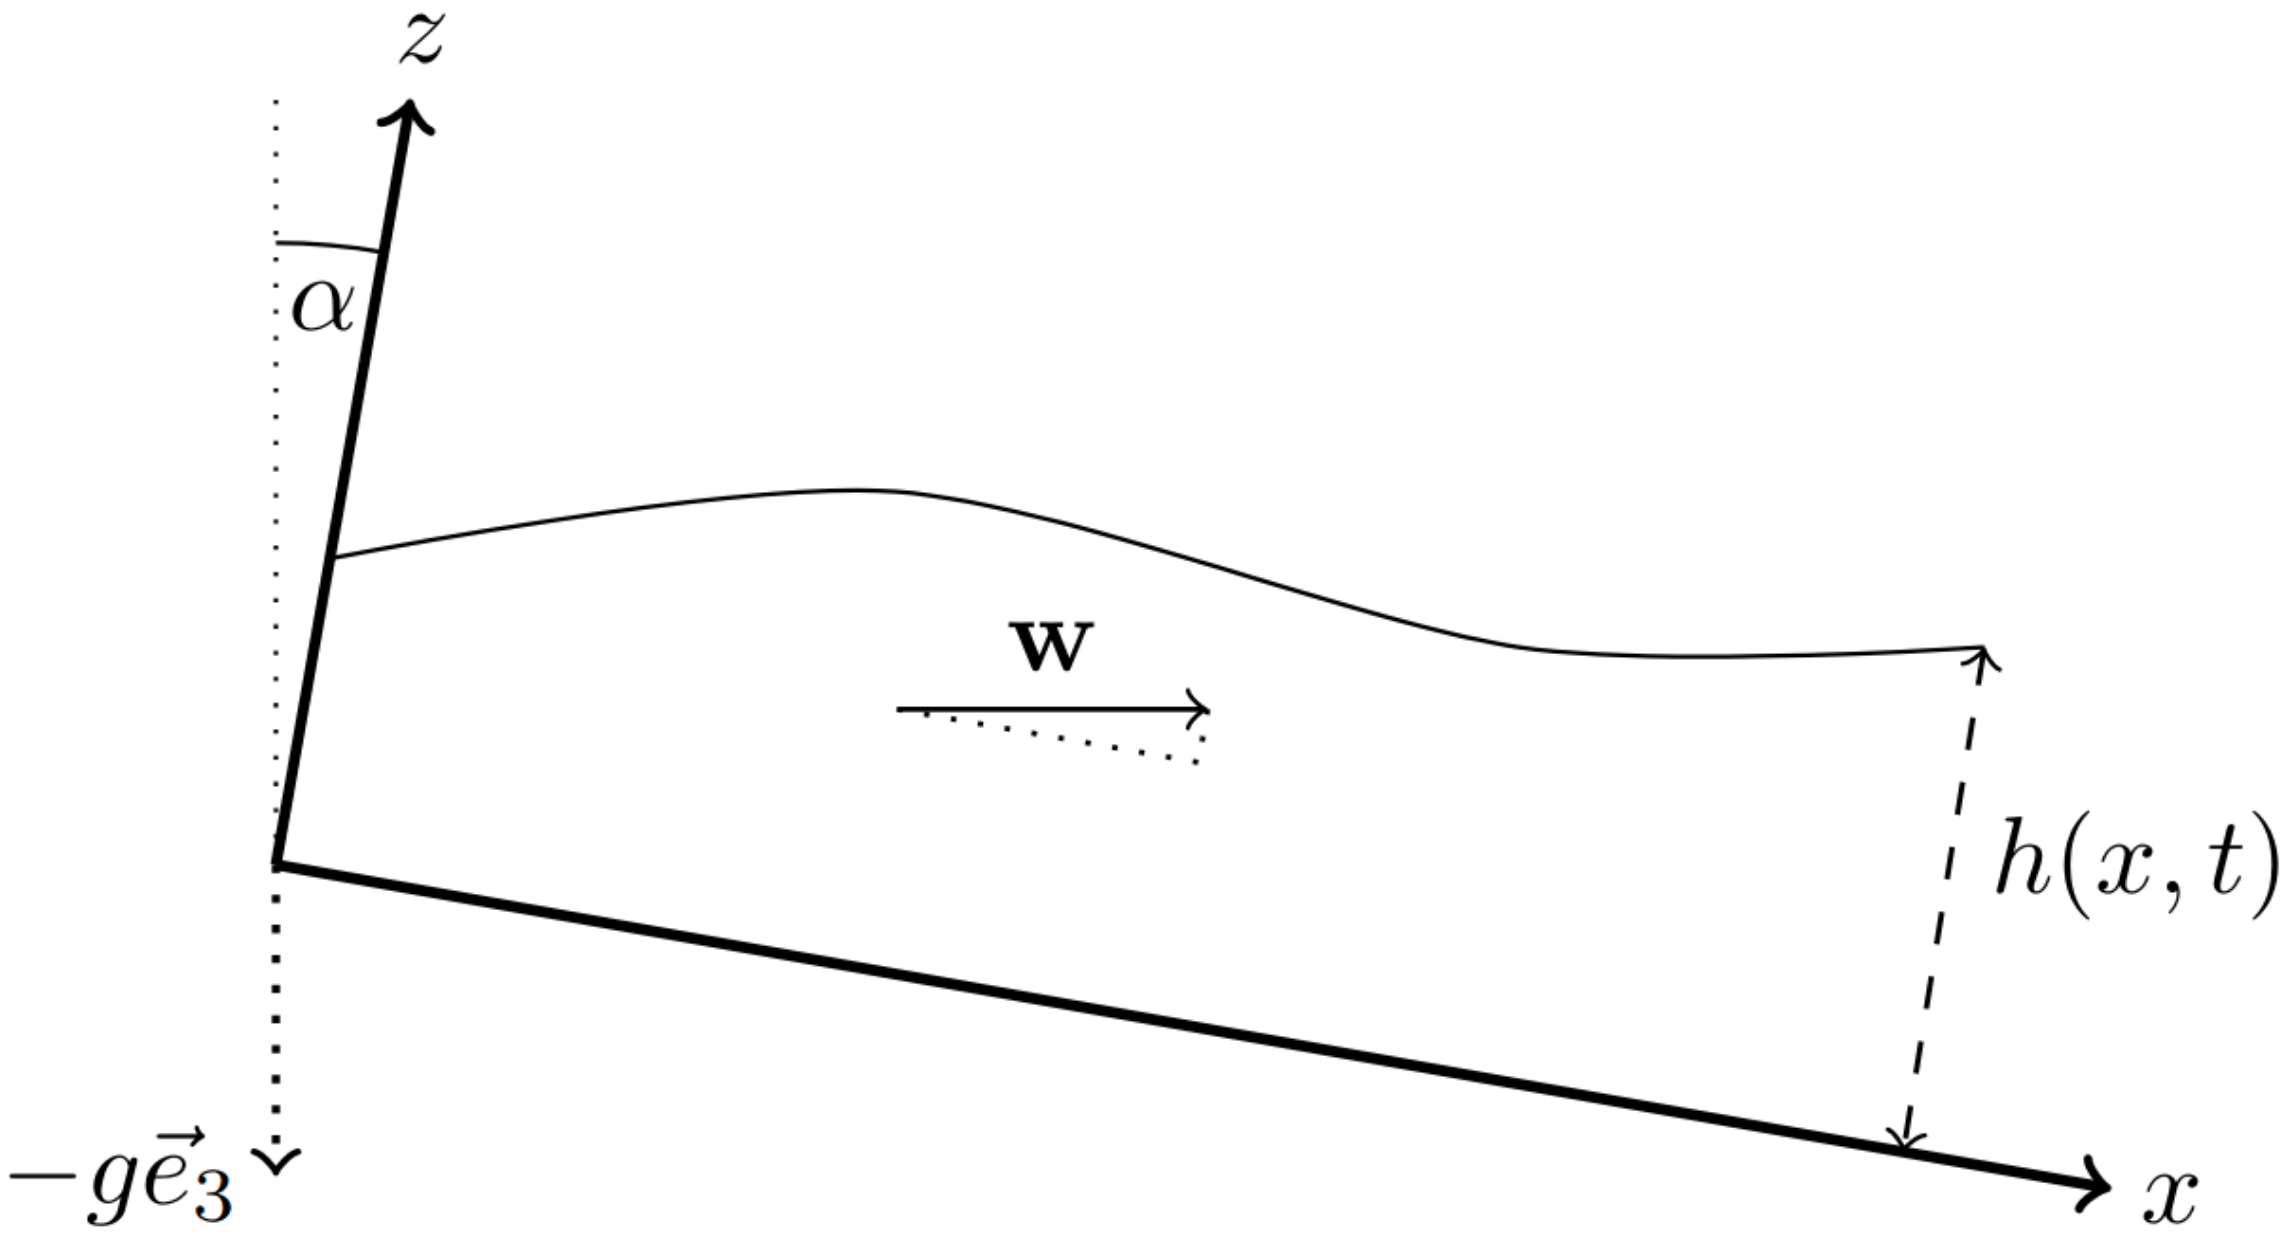
\includegraphics[width=0.5\textwidth]{images/coordinate_system.png}
  \caption{Sketch showing the coordinate system of the glacier. $\alpha$ denotes the slope of the valley floor, $h = h(x, t)$ the glacier's perpendicular height above the valley, and $\vec{w} = (u, v)$ its velocity in $x$ and $z$ directions, respectively \cite{project-description}.}
  \label{fig:coordinate_system}
\end{figure}

Based on conservation of mass and momentum we will formulate equation that describe the relationship between the height of glacier and the velocity within. 